\section{The problem}

\par
As early as 1783, invisible structures in the universe have been hypothesised, but it wasn't until the end of the 19th century, when astronomical photography was realised, that observations gave a hint of an invisible mass \cite{History_Of_Dark_Matter_2018_ref}.
These have grown from humble beginnings as a puzzling curiosity that could perhaps be explained away by observational uncertainties to a direct challenge to fundamental particle physics, cosmology and astrophysics.
In this section, an overview of the evidence for dark matter is given.

%Some other quotes like
%\par
%Perhaps the most fitting conclusion to this was by Lord Kelvin who concluded
%
%\begin{quote}
%    many of our stars, perhaps a great majority of them, may be dark bodies
%\end{quote}
%
% Add Quote about black holes 17XX :P 


\subsection{Galactic Scale}

\par
Some of the earliest indications of dark matter come from comparing methods used to estimate the mass of astronomical bodies.
One such example of this comes from Zwicky who in 1933 sought to determine the mass of the Coma Cluster by relating the potential energy to the kinetic energy using the Virial theorem \cite{Fritz_Zwicky_1933_ref}.
Zwicky found that in order to achieve the average observed velocity of 1000 km/s, there would need to be in excess of $\backsim$12 times more mass than estimated using the galaxy radius and 400 times the mass estimated from luminous matter.
This led him to the conclusion that:
\begin{quote}
``If this should be verified, it would lead to the surprising result that dark matter
exists in much greater density than luminous matter."
\end{quote}
Although this is not the first time the phrase ``dark matter" had been used, it is perhaps the most well-known instance.
Other studies around the same time came to similar conclusions \cite{hubble_and_co_viral_theorem_ref}.
More modern techniques have found issues with these calculations, but the most significant finding of there existing some missing mass remains \cite{a_second_history_of_dark_matter_ref}.

\par
Shortly after, in 1941, it was shown that galactic rotation curves could be used as a reliable way of determining the mass distribution within a galaxy \cite{Chandrasekhar_1941_ref}.
From standard Newtonian dynamics, an object in circular motion with mass $m$ has rotation velocity $v$ that follows:
\begin{equation}
    v(r) = \sqrt{\frac{rF}{m}} = \sqrt{\frac{GM(r)}{r}}
    \label{eq:Kepler_Motion}
\end{equation}
where $G$ is the gravitational constant and $M(r)$ is the mass contained within the radius $r$ given by; $M(r) = 4 \pi \int \rho(r) r^{2} dr$.
\par
In a spiral galaxy, the luminous mass is distributed as approximately a disc. 
Using this, we expect the tangential velocity of an object within the galaxy to increase with the radius until there is equal mass pulling in as there is out.
After this point, the velocity of the object should decrease as $\sqrt{\frac{1}{r}}$ as it becomes further away from the majority of the mass.
However, observations have shown that this is, in fact, not the case, and instead, the velocity distribution remains flat as illustrated in \autoref{fig:DM_Evidence_NGC_6503}.
\begin{figure}[]%
    \centering
    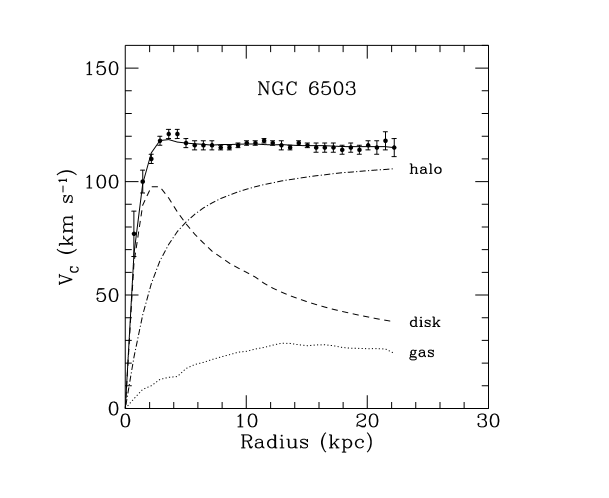
\includegraphics[scale=1.0]{Figures/DarkMatterEvidence/NGC_6503_galaxy_speed.png}
    \caption[Galaxy rotation curve for the NGC 6503 galaxy]{Galaxy rotation curve for the NGC 6503 galaxy along with different mass distribution models which together produce the fit on the observed data. The measurements are from 1991. Figure adapted from \cite{NGC_6503_galaxy_rotation_ref}}
    \label{fig:DM_Evidence_NGC_6503}
\end{figure}
These measurements have been performed multiple times and redone with modern measurements, but always producing results inconsistent with the majority of the mass being in the luminous disc.
Instead, what is suggested is that there is an invisible halo which has a mass density following $\rho(r) \propto \frac{1}{r^2}$ at large $r$.
This remains a topic of ongoing research which now focuses on Low Surface Brightness galaxies, where dark matter is the dominating component \cite{MHONGOOSE_2018_ref}.


\subsection{Galaxy Cluster Scale}
\par
At a larger scale, the discrepancy between the luminous mass and the inferred mass becomes even more apparent.
The general theory of relativity tells us that space-time is warped by the presence of mass.
As such, light propagating along null-geodesics will curve when near any object with mass, with the magnitude of the curvature being directly correlated to the intervening object's mass.
This effect, known as gravitational lensing, can be categorised as strong, weak or microlensing\footnote{Strong lensing typically produces multiple images of the same object. Weak lensing has no noticeable distortion but can be discovered statistically. Microlensing is when a significantly smaller object produces a distortion.}. 
Gravitational lensing manifests itself in observations as duplicate features and distortions.
An example of strong lensing is where light from a distant galaxy has been distorted into an arc due to the mass of an intervening galaxy, once such example is in \autoref{fig:DM_Evidence_Einstein_Ring}  where a near-perfect ring is observed.
A complete catalogue of these can be found in \cite{einstein_ring_discovery_ref}.

\begin{figure}%
    \centering
    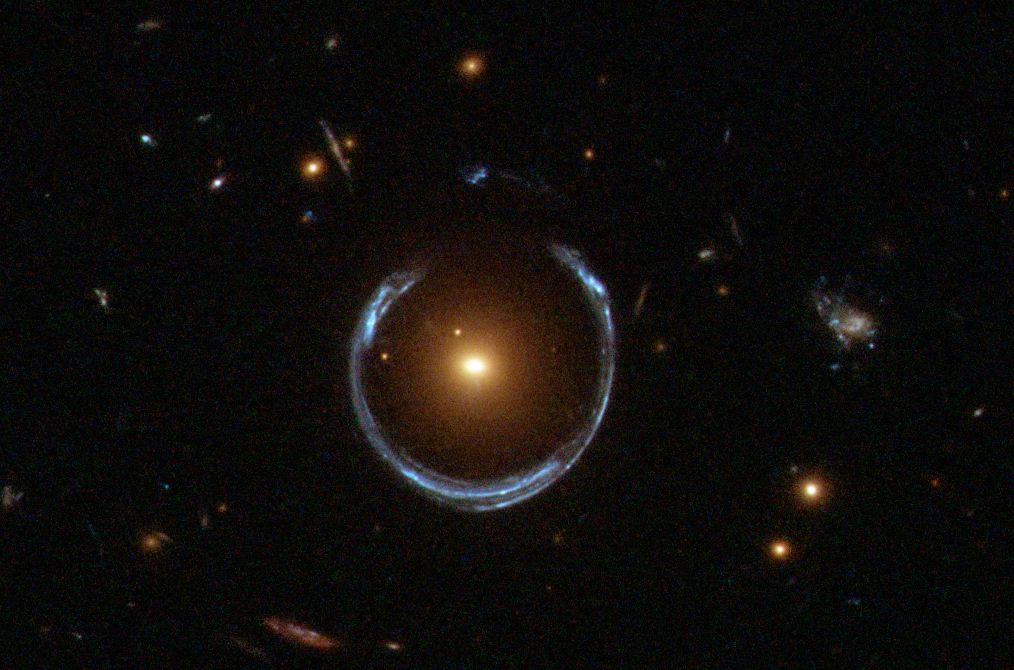
\includegraphics[scale=0.4]{Figures/DarkMatterEvidence/Einstein_Ring_from_Hubble.JPG}
    \caption{An example of a ``Horseshoe Einstein Ring" created by the bending of light from a distant blue galaxy by the central red galaxy LRG 3-757 [ESA/Hubble]}
    \label{fig:DM_Evidence_Einstein_Ring}
\end{figure}

\par
Based on the amount of distortion, the mass of the object causing the lensing can be measured and can be applied to both individual galaxies as well as clusters.
The mass required for the lensing observed can then be compared to the luminous mass, which also shows a mismatch between the two \cite{History_Of_Dark_Matter_2018_ref}.


\par
At the galactic cluster scale, there is yet more evidence of the missing mass, which is easiest to see with the galactic cluster 1E0657-558, also known as the Bullet Cluster.
This galaxy cluster was formed by the merger of two smaller clusters \cite{bullet_cluster_ref}.
In the resultant Bullet Cluster, the baryonic matter can be tracked via electromagnetic radiation and the mass via lensing.
Observations show that there is a discrepancy between the centre of mass from energy and the centre of mass from radiation.
This is shown in \autoref{fig:DM_Evidence_Bullet_Cluster}.
The luminous matter from each of the smaller clusters mixed, causing the matter to slow down.
On the other hand, the majority of the mass has passed through without interacting.
What this indicates is that in addition to there being a significant invisible mass, this mass must also have a very small interaction cross-section with baryonic matter and with itself.

\begin{figure}%
    \centering
     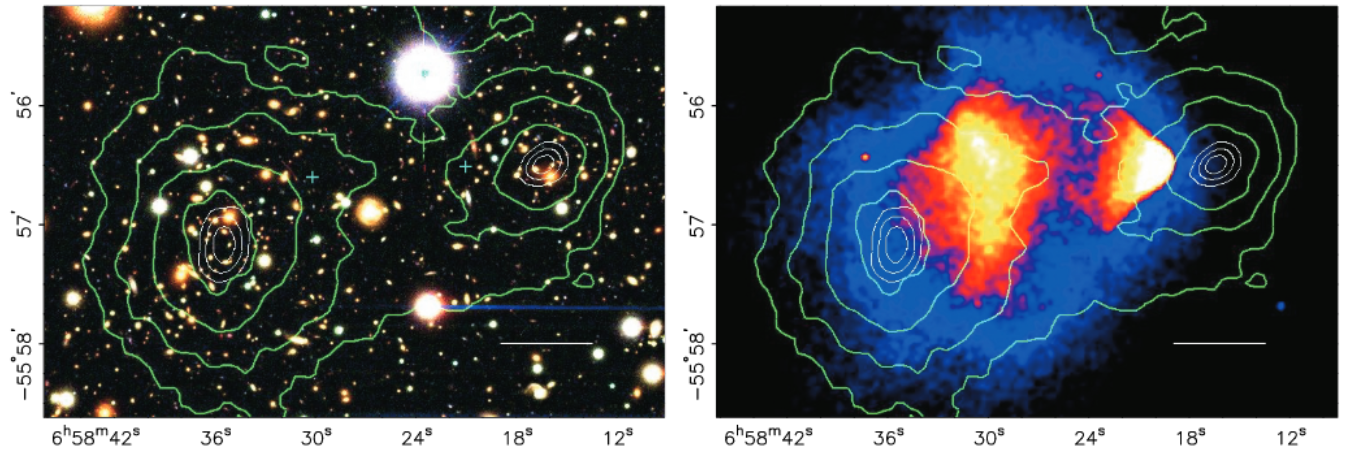
\includegraphics[width=\textwidth]{Figures/DarkMatterEvidence/bullet_cluster_2.png}
    \caption[Merging of two galaxy cluster, 1E 0657-558]{Merging of two galaxy clusters: The Bullet Cluster, 1E 0657-558.
             During the collision, the dark matter components passed through without interacting.
             The baryonic components from the two clusters interacted, causing them to lag behind.
             \textbf{Left:} Optical image from the Magellan observatory.
             \textbf{Right:} X-ray image from the Chandra observatory.
             In both figures, the white bar indicates 200 kpc, the green contours are the mass distribution from weak-lensing reconstructions, and the white contours are the errors in the position of the lensing peaks.
             Figure adapted from \cite{bullet_cluster_ref}.}
    \label{fig:DM_Evidence_Bullet_Cluster}
\end{figure}


\subsection{Cosmological Scale}

\par
What is often quoted as the strongest evidence for dark matter comes from the cosmic microwave background (CMB) radiation which was first discovered in 1965 \cite{cmb_origins_ref}.
This is a near perfectly uniform field of microwave photons with the energy spectrum of a 2.7225 K blackbody, a map of which is shown in \autoref{fig:DM_Evidence_CMB_Map}.
These photons, sometimes referred to as `relic' radiation, last interacted with the early universe when the temperature was almost 3000 K \cite{bigbang_nucleosynthesis_ref}.
This was some 380,000 years after the Big Bang\footnote{The surface of last scattering}, before the universe cooled sufficiently for recombination\footnote{When electrons were first able to bind to nuclei} and neutral Hydrogen formation.
At this time, the universe was filled with plasma as there was enough energy to ionise an atom as soon as it had been formed.
The CMB photons decoupled from the plasma during this time and were able to free-stream through the universe.
As the universe has expanded, these photons have red-shifted down to the now observed microwave photons, and give an insight into the early universe\footnote{It has also been quoted as ``a selfie of the baby universe" \cite{marisarthurs_thesis_ref}}.

\begin{figure}[]%
    \centering
    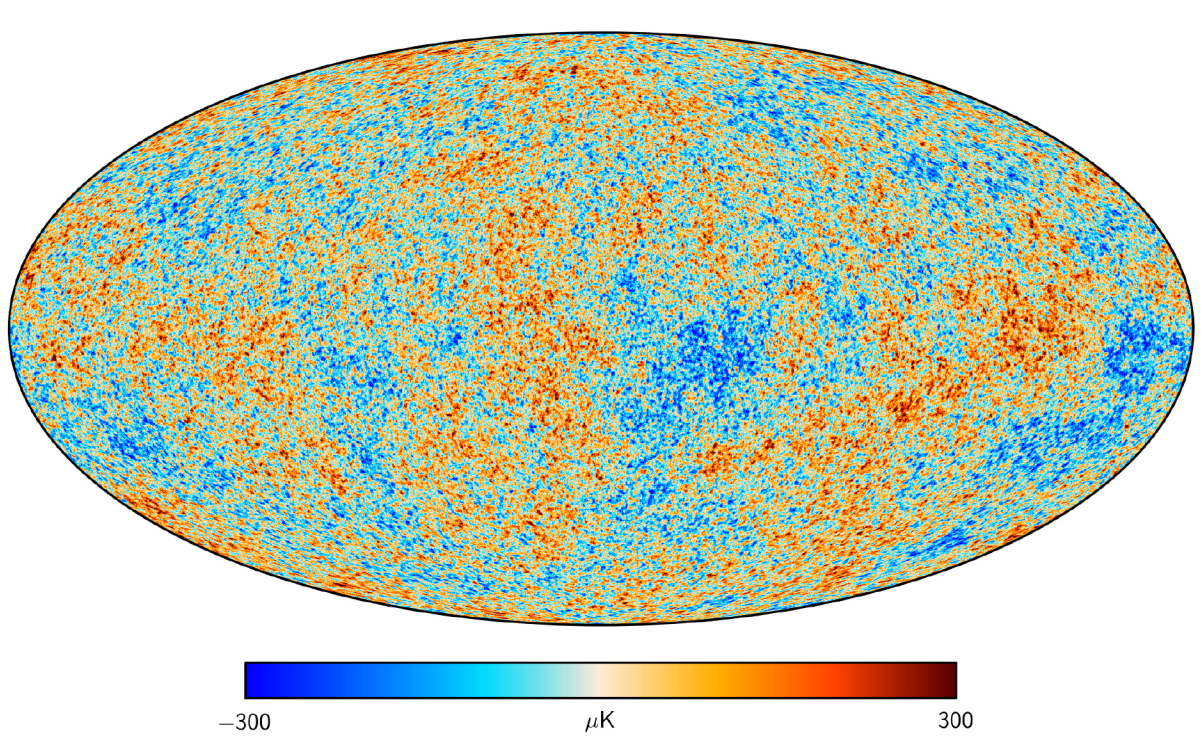
\includegraphics[width=0.8\textwidth]{Figures/DarkMatterEvidence/cmb_radiation.png}
    \caption[Temperature fluctuations of the CMB radiation]{Temperature fluctuations of the CMB radiation from Planck.
             The maximum difference between the warmest (red) and coldest (blue) is 0.0006K.
             Figure from \cite{plank_result_ref}.}
    \label{fig:DM_Evidence_CMB_Map}
\end{figure}

\par
At the time when the CMB decoupled, the universe was extremely isotropic, which can be seen in the uniformity of the CMB, though there are minor anisotropies.
Prior to recombination, any small non-uniformity in the plasma resulted in a gravitation well, into which all forms of matter were pulled.
The inward force of gravity competed with the outward force from photons, tied with the expanding (and therefore cooling) universe resulted in standing pressure waves in the plasma, referred to as baryon acoustic oscillations (BAO), and the temperature fluctuations seen today.
Describing them as spherical harmonics ($Y_{lm}(\theta,\phi)$), the temperature fluctuations can be written as \cite{History_Of_Dark_Matter_2018_ref}:
\begin{equation}
    \frac{\delta T}{T}(\theta, \phi) = \sum_{l} \sum_{m} a_{lm}Y_{lm}(\theta,\phi)
    \label{eq:bao_spherical_harmonics}
\end{equation}
The temperature fluctuations between two points in the CMB can then be described by:
\begin{equation}
    C(\theta) = \frac{1}{4\pi} \sum_{l} (2l + 1) C_l P_l (cos(\theta))
\end{equation}
where $\theta$ is the angular separation between two points and $P_l (cos(\theta))$ are Legendre polynomials.
$C_l$ can be considered as the magnitude of the temperature fluctuation when $l$ is large, making $l$ a proxy for angular separation.
\par
The application of this on the latest Planck measurement of the CMB is shown in \autoref{fig:DM_Evidence_BAO} \cite{plank_result_ref}.
The shape of the spectrum in \autoref{fig:DM_Evidence_BAO} sets significant constraints on the $\Lambda$CDM model of the universe, the best model that currently exists to describe the universe and galaxy formations.
The observed CMB is best fitted with an energy density in the universe divided up as: 4.88\%$\pm$0.03\% baryonic matter, 26.01\%$\pm$0.22\% dark matter and the remaining 69.11\%$\pm$0.62\% being dark energy \cite{plank_result_ref}.

\begin{figure}%
    \centering
    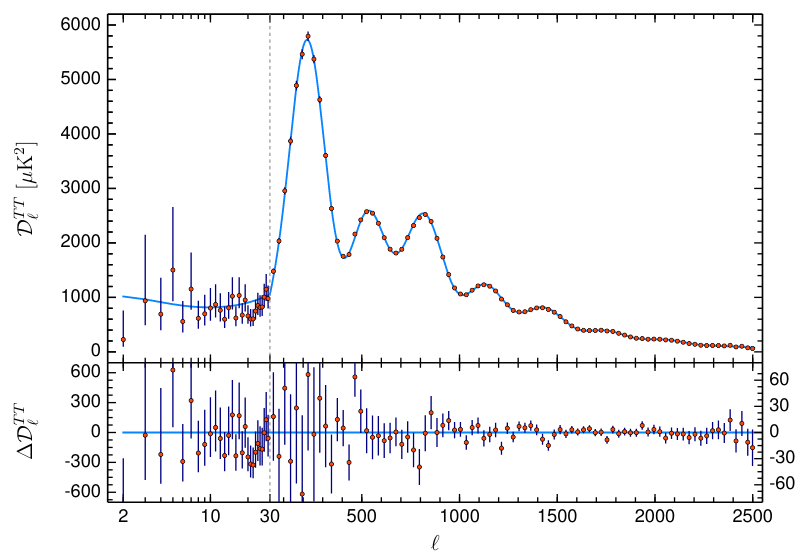
\includegraphics[width=0.8\textwidth]{Figures/DarkMatterEvidence/bao.png}
    \caption[Temperature fluctuations of the CMB spectrum as a function of $l$]{The temperature fluctuations of the CMB power spectrum against the spherical harmonics multipole parameter, $l$, which is a proxy for angular separation.
             \textbf{Top:} the power spectrum fitted to the $\Lambda$CDM model.
             \textbf{Bottom:} the residuals of the fit, shown to be small.
             Figure from \cite{plank_result_ref}.}
    \label{fig:DM_Evidence_BAO}
\end{figure}
